% Compile with pdflatex, xelatex, or tectonic:
%   tectonic report.tex      (recommended; self-contained)
%   pdflatex report.tex      (run twice to resolve references)
\documentclass[11pt]{article}

\usepackage[T1]{fontenc}
\usepackage{lmodern}
\usepackage{graphicx}
\usepackage{booktabs}
\usepackage{geometry}
\geometry{a4paper, margin=2.5cm}
\usepackage{hyperref}
\hypersetup{colorlinks=true, linkcolor=blue, urlcolor=blue}

\title{ERA Tree Search vs.\ Best-of-$N$ Sampling:\\ A Small Local Reproduction}
\author{Reproduction Experiment Log --- Stage 2}
\date{\today}

\begin{document}
\maketitle

\section{Goal}
This is the second stage of reproducing the official
\href{https://github.com/google-research/era}{\texttt{google-research/era}} demo
(for the Nature paper \emph{An AI system to help scientists write expert-level
empirical software}). Stage~1 confirmed that the ERA tree-search loop runs and
improves a solution over iterations. Stage~2 tests a sharper claim from the
paper: that \textbf{ERA is not merely best-of-$N$ sampling} --- its tree search
is supposed to explore the space of programs \emph{more efficiently} than drawing
$N$ independent samples and keeping the best.

\section{Experimental Setup}
Both methods run on the \textbf{same} task, the same local train/test split, and
the same scoring function as \texttt{playground\_s3e1.py} (the
California-Housing-style regression demo). The metric is the
\textbf{negative RMSE} ($-\mathrm{RMSE}$); higher (closer to $0$) is better. Both
methods start from the identical initial solution (a plain linear regression) and
are given an \textbf{equal budget of $N=20$ LLM calls}.

\begin{itemize}
  \item \textbf{ERA tree search (Method A).} Runs the existing FUTS / ERA search
        for $20$ expansions. Each new candidate is generated conditioned on a
        \emph{tree-selected parent}, so promising solutions are built upon.
  \item \textbf{Best-of-$N$ independent sampling (Method B).} Generates $20$
        candidates, each conditioned on the \emph{same} initial solution and
        score. It never conditions on previously generated candidates --- every
        sample is drawn independently from the identical starter prompt, making
        it a fair independent-sampling baseline.
\end{itemize}

Because both methods make exactly $N$ LLM calls, the $x$-axis
(``number of candidate programs evaluated'') is directly comparable.

\section{Results}
Table~\ref{tab:results} summarises the run, and Figure~\ref{fig:compare} shows the
running-best score versus the number of candidates evaluated.

\begin{table}[h]
\centering
\begin{tabular}{lc}
\toprule
\textbf{Quantity} & \textbf{Best score (negative RMSE, higher is better)} \\
\midrule
Initial baseline                 & $-0.7339$ \\
ERA tree search (final best)     & $\mathbf{-0.5735}$ \\
Best-of-$N$ (final best)         & $-0.6149$ \\
\midrule
\textbf{Winner}                  & \textbf{ERA tree search} \\
\bottomrule
\end{tabular}
\caption{Final results after $N=20$ candidates per method (single run).}
\label{tab:results}
\end{table}

\begin{figure}[h]
\centering
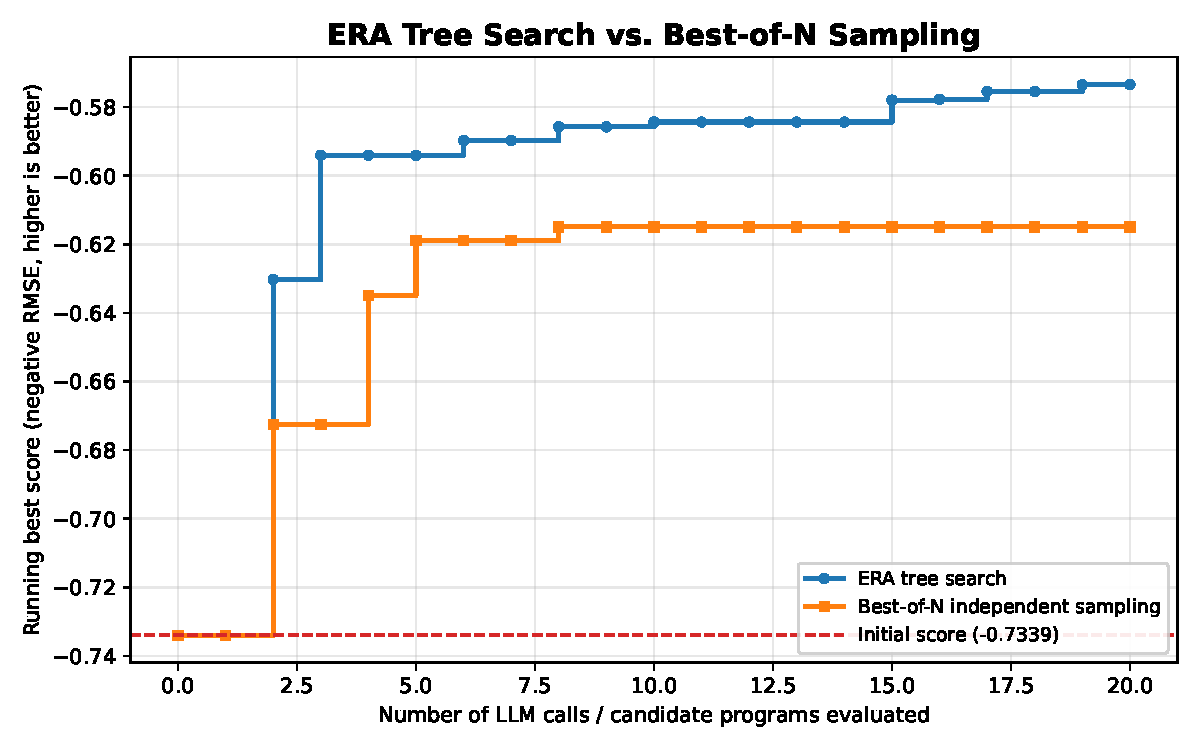
\includegraphics[width=0.85\textwidth]{era_vs_bon}
\caption{Running-best score (negative RMSE) versus number of candidate programs
evaluated. Blue: ERA tree search. Orange: best-of-$N$ independent sampling.
Red dashed line: the shared initial score. Under an equal budget of $20$ LLM
calls, ERA reaches a clearly better solution.}
\label{fig:compare}
\end{figure}

\section{Interpretation}
\begin{itemize}
  \item \textbf{ERA wins under an equal budget.} With the same $20$ LLM calls,
        ERA reached $-0.5735$ while best-of-$N$ plateaued at $-0.6149$, a gap of
        about $0.041$ in RMSE. ERA also keeps improving late in the run, whereas
        best-of-$N$ flattens early.
  \item \textbf{Conditioning on good parents helps twice.} ERA generates each new
        candidate from the \emph{best working solution so far}, so it both (a)
        climbs higher and (b) is far more \emph{reliable}: in this run ERA
        produced only $3/20$ invalid (non-executing) candidates, versus $13/20$
        for best-of-$N$. Best-of-$N$ repeatedly tries to write a complex
        feature-engineered model from scratch off the weak linear baseline, and
        fails more often; ERA instead edits code that already runs.
  \item \textbf{Consistent with the paper's claim.} This miniature experiment
        reproduces, qualitatively, the idea that ERA's tree search is more
        sample-efficient than naive independent sampling --- it is ``not just
        best-of-$N$.''
\end{itemize}

\section{Caveats and Limitations}
\begin{itemize}
  \item \textbf{Single stochastic run.} This is one run with $N=20$. LLM sampling
        is random, so the exact gap will vary; a rigorous claim should average
        several seeds and/or use a larger $N$ with confidence intervals.
  \item \textbf{Toy task.} The California-Housing demo has a small search space
        and plateaus quickly, so absolute gaps are modest.
  \item \textbf{Insecure sandbox.} Candidates are executed via the local
        \texttt{sandbox.py}, which is \emph{not} a secure sandbox (it runs
        LLM-generated code directly). It is used here only for this trusted toy
        reproduction.
\end{itemize}

\section{Next Steps}
\begin{itemize}
  \item Repeat the comparison over several random seeds and report
        mean~$\pm$~standard deviation of the final best score for each method.
  \item Sweep the budget $N$ (e.g.\ $10, 20, 40$) to see how the ERA-vs-best-of-$N$
        gap scales with the number of LLM calls.
  \item Once the gap is robust on the toy task, move toward the fuller scientific
        tasks from the paper.
\end{itemize}

\end{document}
